\documentclass[12pt]{article}

\usepackage{ifpdf}
\ifpdf
\usepackage{cmap}
\usepackage{graphicx}
\graphicspath{{pictures/}}
\DeclareGraphicsExtensions{.pdf,.png,.jpg,.bmp}
\usepackage[unicode=true]{hyperref}
\else
\usepackage[dvips]{graphicx}
\fi
\usepackage[utf8]{inputenc}
\usepackage[T2A]{fontenc}
\usepackage[russian]{babel}
\usepackage{mathtext}
\usepackage{latexsym}
\usepackage{amsthm}
\usepackage{calc}
\usepackage{hhline}
\usepackage{colortbl}
\usepackage{comment}
\usepackage{fancybox}
\usepackage{hyperref}
\usepackage[14pt]{extsizes}
\usepackage{amssymb,amsfonts,amsmath,cite,enumerate,float,indentfirst,xcolor}

\usepackage{amsmath, amssymb, amsthm}
\usepackage{mathtext}
\usepackage{mathenv}
\numberwithin{equation}{section}

\begin{document}

\tableofcontents
\clearpage

\section{Введение}
В этой работе рассмотрена качающаяся машина Атвуда, в которой один из грузов может совершать движения в двумерной плоскости (рис. \ref{atwood}). Блоки не имеют массы и трения, веревка не растяжима и также не имеет массы. Предполагается, что веревка достаточно длинная, чтобы противовес $M$ не касался блока, с другой стороны мы даем качающемуся грузу $m$ подниматься над горизонтальной линией и делать полные обороты вокруг блока, полагая, что веревка всегда остается в натяжении.

\begin{figure}[H]
    \centering
    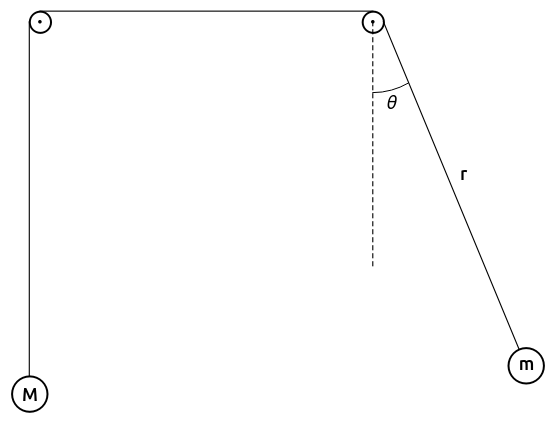
\includegraphics[width=11cm]{atw.png}
    \caption{Качающаяся машина Атвуда.}
    \label{atwood}
\end{figure}



\section{Теория}
\subsection{Уравнения движения}
Качающаяся машина Атвуда имеет две степени свободы. В качестве координат возьмем $r$ и $\theta$, которые обозначены на рис. \ref{atwood}. Кинетическая энергия системы:
\begin{equation}\label{f1}
T=\frac{1}{2}M\dot{r}^{2}+\frac{1}{2}m (\dot{r}^{2}+r^{2}\dot{\theta}^{2}),
\end{equation}
потенциальная энергия системы (без произвольной постоянной):
\begin{equation}\label{f2}
V=gr(M-m \cos \theta),
\end{equation}
где $g$ -- ускорение свободного падения. Функция Лагранжа системы ($L=T-V$), в таком случае, имеет вид:
\begin{equation}\label{f3}
L=\frac{1}{2}M\dot{r}^{2}+\frac{1}{2}m (\dot{r}^{2}+r^{2}\dot{\theta}^{2})+gr(m \cos \theta-M).
\end{equation}

Получим уравнения Эйлера-Лагранжа ($ \frac{d}{dt}(\frac{\partial L}{\partial \dot{q}_{i}}) = \frac{\partial L}{\partial q_{i}} $):
\begin{equation}\label{f4}
с\begin{cases}
(m+M)\ddot{r} = m r \dot{\theta}^{2}+g(m \cos\theta - M),\\
\frac{d}{dt}(mr^{2}\dot{\theta})=-mgr\sin\theta.\\
\end{cases}
\end{equation}

Первое уравнение системы $\ref{f4}$  — закон Ньютона в радиальном направлении. Второе уравнение говорит о том, что скорость изменения углового момента равна моменту силы тяжести.

Для упрощения определим:
\begin{equation}\label{f5}
\mu=\frac{M}{m}.
\end{equation}

Тогда система $\ref{f4}$ примет окончательный вид:
\begin{equation}\label{f6}
\begin{cases}
(1+\mu)\ddot{r} = r \dot{\theta}^{2}+g( \cos\theta - \mu);\\
r\ddot{\theta}+2 \dot{r} \dot{\theta}+ g \sin\theta=0.\\
\end{cases}
\end{equation}

Движение качающейся машины Атвуда полностью описывается системой $\ref{f6}$ и начальными условиями:
\begin{equation}\label{f7}
\begin{cases}
r(0)=r_{0}\\
\theta(0)=\theta_{0}\\
\dot r(0)=\dot r_{0}\\
\dot \theta(0)=\dot \theta_{0}\\
\end{cases}
\end{equation}
\subsection{Закон сохранения энергии}
Поскольку диссипативные силы отсутствуют, энергия системы
\begin{equation}\label{f8}
E=T+V=\frac{1}{2}M\dot{r}^{2}+\frac{1}{2}m (\dot{r}^{2}+r^{2}\dot{\theta}^{2})+gr(M-m \cos \theta)
\end{equation}
сохраняется.

Это можно также понять из функции Лагранжа системы, поскольку $ \frac{\partial L}{\partial t} = 0 $.

\subsection{Поведение системы}

В зависимости от начальных условий и отношения масс $ \mu $, качающаяся масса описывает различные виды траекторий. Классифицируем их (с иллюстрациями из программы):
\clearpage
\begin{enumerate}
	\item \textbf{Ограниченная траектория} (рис. \ref{finite}): $ \;\; r(t)<r_{max}\;\; \forall \;t\geqslant0. $\\ 
	Траектория ограничена, если $ M>m $. Доказательство этого факта приведено в статье \cite{bib1} 
	\vspace{2em}
	\begin{figure}[h]
		\center{
			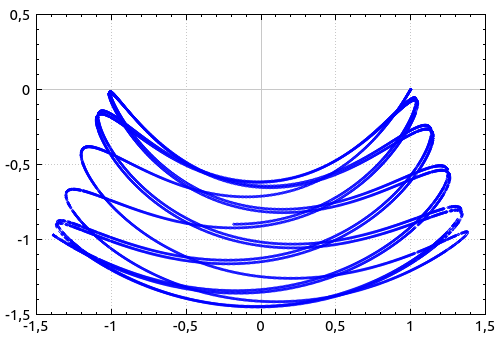
\includegraphics[scale=0.55]{1.4_1.5708}
			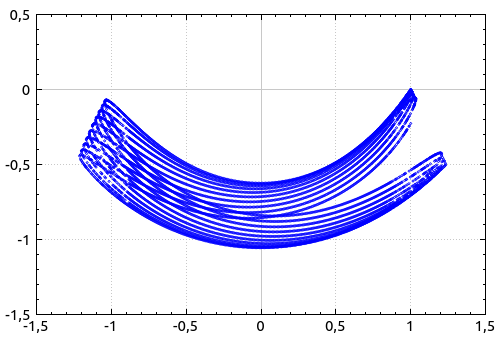
\includegraphics[scale=0.55]{1.5_1.5708}
			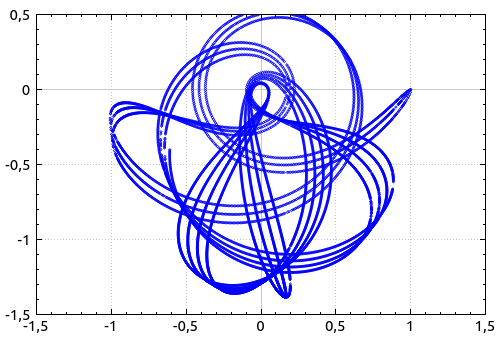
\includegraphics[scale=0.55]{3.5_1.5708}
			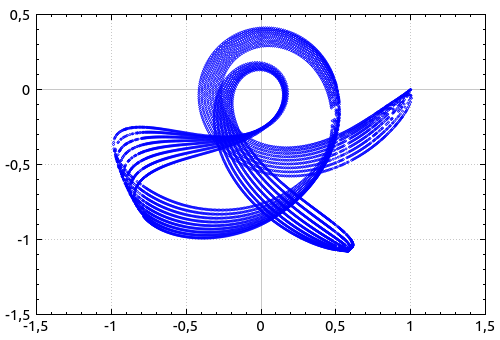
\includegraphics[scale=0.55]{4.8_1.5708}
		}
		\caption{Ограниченные (и несингулярные) траектории при ${\mu=1.4;\;1.5;\;3.5;\;4.8}\;\;$ и $\;\; \theta_{0}=\pi/2 $}
        \label{finite}
	\end{figure}
	\clearpage
	\item \textbf{Периодическая траектория} (рис. \ref{periodic}): \\ $\exists\tau:\;\; r(t+\tau)=r(t),\;\;\theta(t+\tau)=\theta(t)\;\;\; \forall \;t\geqslant0 .$\\
	\vspace{3em}
	\begin{figure}[h]
		\center{
			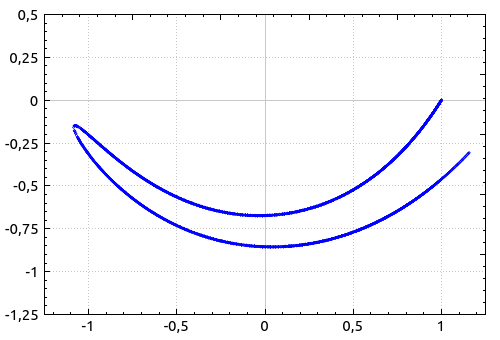
\includegraphics[scale=0.55]{1.555_1.5708}
			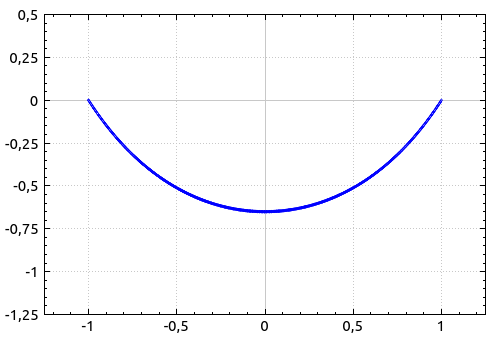
\includegraphics[scale=0.55]{1.665_1.5708}
			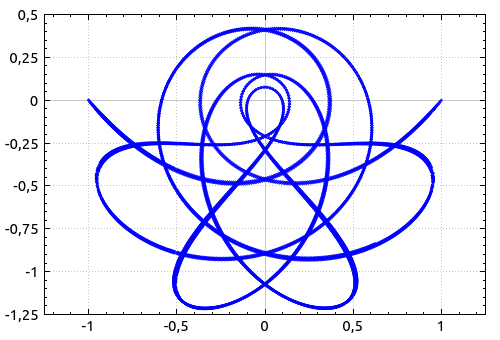
\includegraphics[scale=0.55]{4.175_1.5708}
			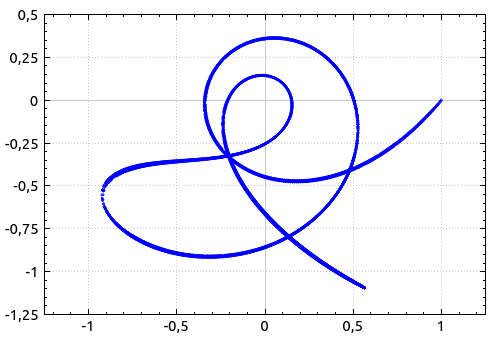
\includegraphics[scale=0.55]{4.745_1.5708}
		}
		\caption{Периодические траектории при $\mu=1.555;\;1.665;\;4.175;\;4.745$ и $\; \theta_{0}=\pi/2 $}
        \label{periodic}
	\end{figure}
	\clearpage
	\item \textbf{Сингулярная траектория} (рис. \ref{singular}): $ r(0)=0. $\\
	Будем называть траекторию сингулярной, если в какой-либо точке $ r $ обнуляется. Чтобы получить такую траекторию можно просто установить начальное значение $ r(0) = 0 $. Но поскольку система инвариантна относительно трансляций во времени мы всегда можем организовать всё так, что любая сингулярная траектория начинается в точке $ r(0) = 0 $.
	\vspace{2em}
	\begin{figure}[h]
		\center{
			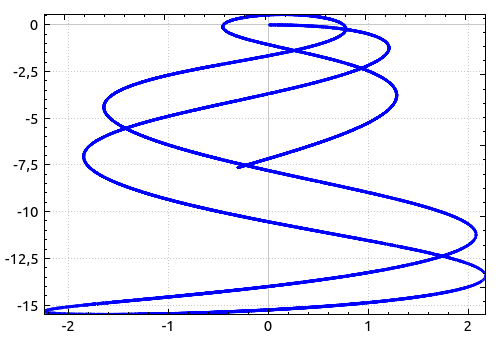
\includegraphics[scale=0.55]{1.1_1.5708}
			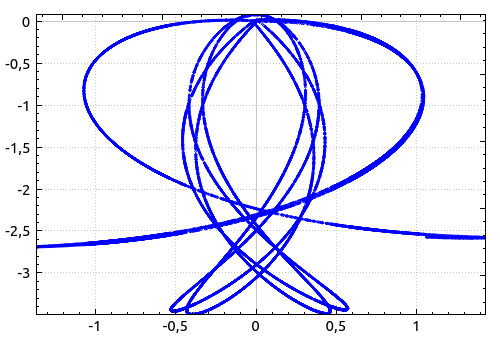
\includegraphics[scale=0.55]{1.6_1.5708}
			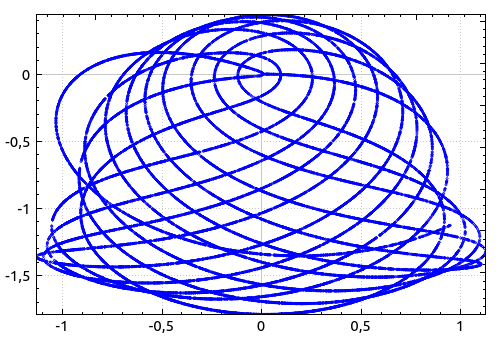
\includegraphics[scale=0.55]{2.3_1.5708}
			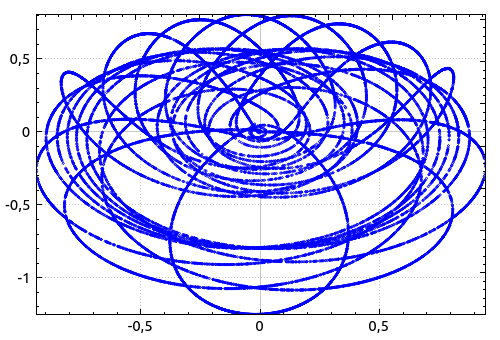
\includegraphics[scale=0.55]{4.6_1.5708}
		}
		\caption{Сингулярные траектории при $ \mu=1.1;\;1.6;\;2.3;\;4.6 $ , $\;\;\;\;\;\;\;\; \theta_{0}=\pi/2, \;\; \dot r(0) = 4.$}
        \label{singular}
	\end{figure}
	\clearpage
	
	\item \textbf{Прекращающаяся сингулярная траектория} (рис. \ref{terminating}):\\ $ \exists\tau>0: \;\; r(\tau)=r(0)=0 $ 
	\begin{figure}[h]
		\center{
			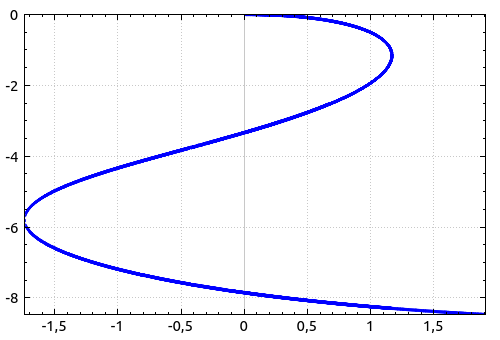
\includegraphics[scale=0.5]{1.182_1.5708}
			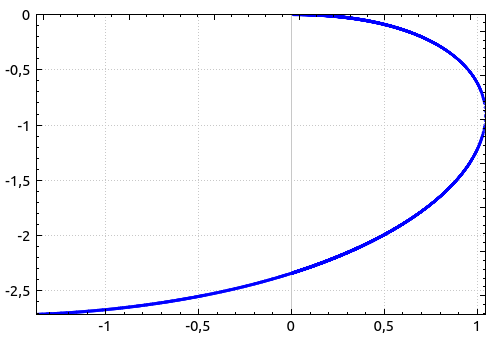
\includegraphics[scale=0.5]{1.594_1.5708}
			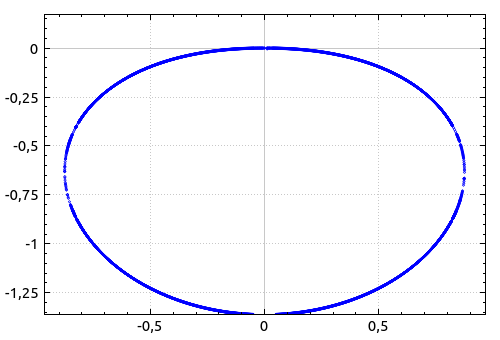
\includegraphics[scale=0.5]{3_1.5708}
			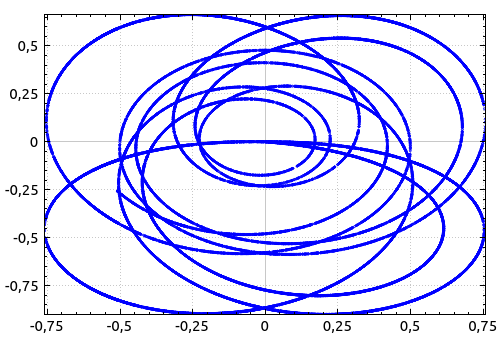
\includegraphics[scale=0.5]{8.13_1.5708}
		}
		\caption{Прекращающиеся сингулярные траектории при ${\mu=1.182;\;1.594;\;3;\;8.120}$, $\;\;\theta_{0}=\pi/2, \;\; \dot r(0) = 4.$}
        \label{terminating}
	\end{figure}	
\end{enumerate}
\section{Описание программы}

В процессе работы программы происходит численное интегрирование предложенной системы дифференциальных уравнений методом Рунге -- Кутты четвертого порядка. В интерфейсе программы можно задавать значения параметров и наблюдать построение траектории, фазовых плоскостей и график относительной энергии системы.
\subsection{Метод решения}
Преобразуем уравнения \ref{f6}, введя новые переменные: $ p(t)=\dot r(t) $, $ q(t)=\dot \theta(t)$. Тем самым мы придем к системе из четырех уравнений, разрешенных относительно производной: 
\begin{equation}\label{fk}
\begin{cases}
\dot r = p\\
\dot \theta = q\\
\dot{p} =\frac{1}{(1+\mu)}( r \,q^{2}+g( \cos\theta - \mu))\\
\dot q=\dfrac{1}{r}(2\,p\,q-g sin\theta).\\
\end{cases}
\end{equation}
С начальными условиями:
\begin{equation}\label{fn}
\begin{cases}
r(0)=r_{0}\\
\theta(0)=\theta_{0}\\
p(0)=\dot r_{0}\\
q(0)=\dot \theta_{0}\\
\end{cases}
\end{equation}
Для численного решения этой системы был применен метод Рунге-Кутты 4-го порядка.
\subsection{Интерфейс программы}
\begin{figure}[h]
	\center{
		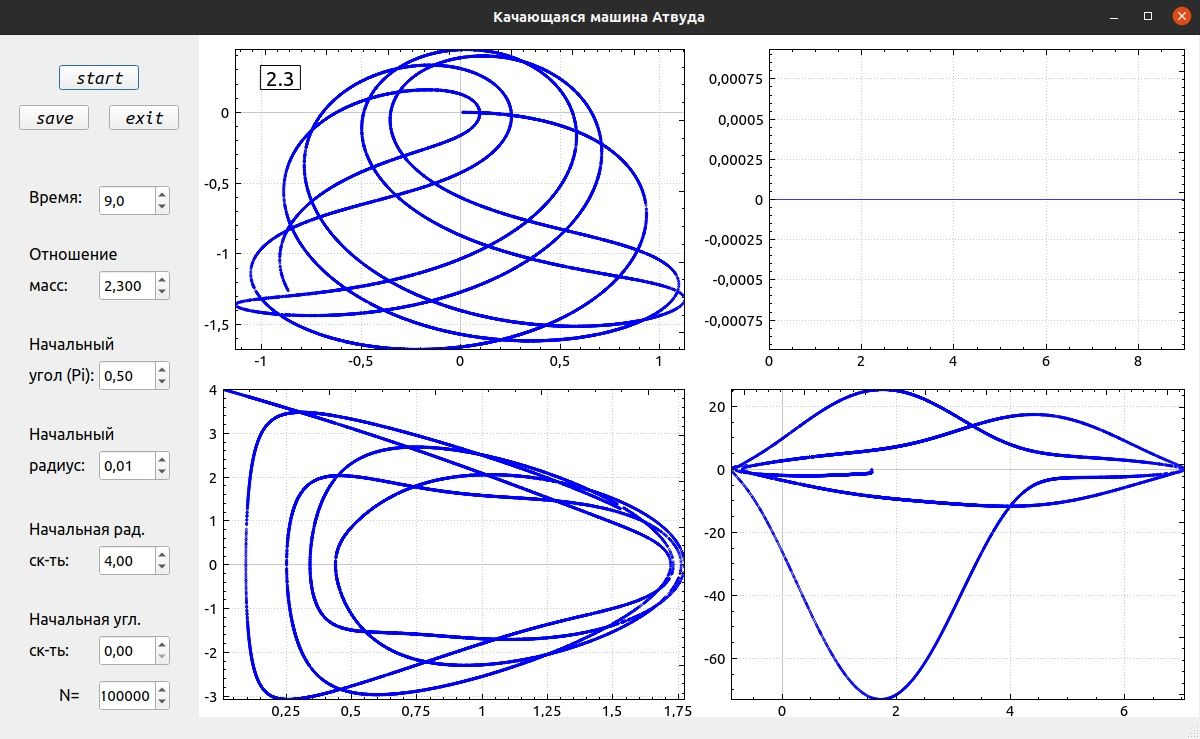
\includegraphics[scale=0.36]{gui.png}
	}
	\caption{Окно программы.}
    \label{menu}
\end{figure}

\textbf{Параметры, которые можно задавать в меню программы (рис. \ref{menu}):}
\begin{enumerate}
	\item число шагов;
	\item время движения;
	\item отношение масс грузов;
	\item начальный угол;
	\item начальная длина нити;
	\item начальная радиальная скорость;
	\item начальная угловая скорость;
\end{enumerate}
\textbf{Графики, строящиеся в результате выполнения программы:}
\begin{enumerate}
	\item график траектории движения груза (слева сверху)
	\item график зависимости относительного изменения энергии \\$ \;\;\epsilon(t)=|100*\frac{E(t)-E(0)}{E(0)}| $ от времени $ t $ (справа сверху)
	\item фазовый портрет №1: зависимость $ \dot r (t) $ от $ r (t) $ (слева внизу)
	\item фазовый портрет №2: зависимость $ \dot \theta (t) $ от $ \theta (t) $ (справа внизу)
\end{enumerate}

Помимо этого в программе есть возможность сохранить полученные графики в формате PNG по нажатию кнопки "save".
\section{Итоги работы}
В ходе выполнения проекта: 
\begin{enumerate}
	\item Написана программа выполняющая численное решение системы дифференциальных уравнений, описывающих качающуюся машину Атвуда, методом Рунге--Кутты 4-го порядка.
	\item Исследованы различные типы траекторий движения груза. Получены графики этих траекторий и фазовые портреты.
	\item Достоверность полученных решений подтверждают графики относительной энергии, которые также строятся в программе.
\end{enumerate}
\clearpage

\begin{thebibliography}{3}
\bibitem{bib1}
B. Tuffilaro, A. Abbot,  and J. Griffits. Atwood’s machine. American Journal of Physics, doi: 10.1119/1.13791, 1984.
\bibitem{ll}
Л. Д. Ландау и Е. М Лифшиц. Теоретическая физика: Т.I Механика. Издательство Наука. 1988. --- 216 c.
\bibitem{nef}
Нефедов Н.Н., Попов В.Ю., Волков В.Т. Обыкновенные дифференциальные уравнения. Курс лекций — М.: Физический факультет МГУ им. М.В. Ломоносова, 2016. — 200 с.
\end{thebibliography}

\clearpage
\end{document}